%課題研究レジュメテンプレート ver. 1.2

\documentclass[uplatex]{jsarticle}
\usepackage[top=20mm,bottom=20mm,left=20mm,right=20mm]{geometry}
\usepackage[T1]{fontenc}
\usepackage{txfonts}
\usepackage{wrapfig}
\usepackage[expert,deluxe]{otf}
\usepackage[dvipdfmx,hiresbb]{graphicx}
\usepackage[dvipdfmx]{hyperref}
\usepackage{pxjahyper}
\usepackage{secdot}

\makeatletter
  \renewcommand{\section}{%
    \if@slide\clearpage\fi
    \@startsection{section}{1}{\z@}%
    {\Cvs \@plus.5\Cdp \@minus.2\Cdp}% 前アキ
    {.5\Cvs \@plus.3\Cdp}% 後アキ
    %{\normalfont\Large\headfont\raggedright}}
    {\normalfont\raggedright}}

  \renewcommand{\subsection}{\@startsection{subsection}{2}{\z@}%
    {\Cvs \@plus.5\Cdp \@minus.2\Cdp}% 前アキ
    {.5\Cvs \@plus.3\Cdp}% 後アキ
    %{\normalfont\large\headfont}}
    {\normalfont}}

  \renewcommand{\subsubsection}{\@startsection{subsubsection}{3}{\z@}%
    {\Cvs \@plus.5\Cdp \@minus.2\Cdp}%
    {\z@}%
    %{\normalfont\normalsize\headfont}}
    {\normalfont}}
\makeatother
%ここから上を編集する必要はない.




\title{\vspace{-14mm}津田沼祭における来場者数の予測式の作成}
\author{PMコース 矢吹研究室 1342045 川手 元稀}
\date{}%日付を入れる必要はない.
\pagestyle{empty}%ページ番号は振らない.
\begin{document}
\maketitle




\section{研究の背景}

私がこの研究に着手した背景が2つある.

1点目に私は大学祭実行委員会に所属している.毎年,実行委員会では来場者数を計測している.2015年度の来場者数は過去最大数になりますます盛り上がることが期待されている.しかし,来場者数が増加することで事故,傷害といったリスクが高まる.
例えば,過去にあった事例だと人が多すぎてステージ前で将棋倒しになり,負傷者を出したことや人通りが多く子どもが迷子になることなど様々である.そこで,来場者数を事前に予測して過去に同じような来場者数が出ている年を参考に事故のリスクを予測・対応ができないかと考えた.

2点目に大学祭実行委員の労働時間の長さである.受付,警備は9時間もの間行わなければならない.過酷な労働が原因で体調不良者が出てしまう傾向にある.
そこで,私は来場者数に応じて実行委員を適正人数で運営できることができたら良いと考えた.

%\begin{wrapfigure}[行数]{r}{幅}%行数はオプションだが,調整しないとうまくいかない.
\begin{wrapfigure}[10]{r}{10cm}
\vspace*{-\intextsep}
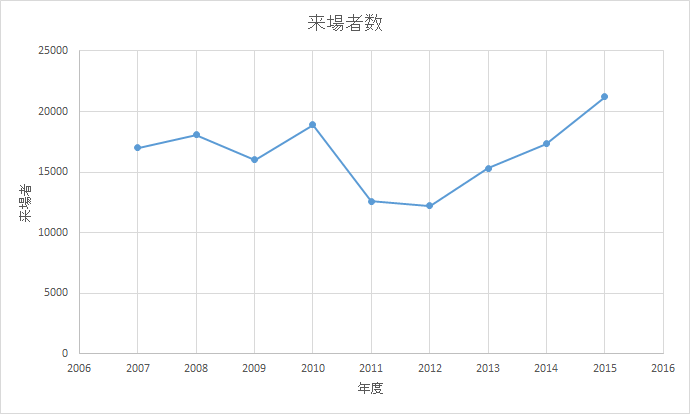
\includegraphics[width=10cm,clip]{raijoushasuu.png}
\caption{津田沼祭来場者数のグラフ}\label{図1}
\end{wrapfigure}


\section{研究の目的}
本研究は3段階に分かれる.

\begin{enumerate}
\item 津田沼祭のブースを運営している人数,開催曜日,天候をベースに来場者数の予測式を立てる.
\item 立てた予測式の整合性を確認する.
\item 予測された来場者数と過去に類似した来場者の年の事件を確認し,事件が起きても対応できるようにする.
\end{enumerate}

\section{プロジェクトマネジメントとの関連}

プロジェクトマネジメントとの関連については以下に記載する.

\begin{enumerate}
\item 人的資源とコストの分野で関連がある.来場者数に応じて警備や受付を適正人数で行えることである.実行委員の仕事を軽減することが可能になり,個人のモチベーションの向上に繋がるからだ.
\item リスクマネジメントの分野で関連がある.来場者を予測することでリスクを洗い出し対応策を過去の事例から考えられるからだ.
\end{enumerate}

\section{研究の方法}

\subsection{データの収集について}

過去9年分の津田沼祭のデータを大学祭実行委員会の許可を取り収集を行った.データ項目は各年代の来場者数,運営人数,開催日,開催曜日である.

天候にも関係があると考え開催日の天候のデータを収集した.\cite{a}

\subsection{データの解析方法}

データの解析方法を以下に記載する.


\begin{enumerate}
\item 開催した曜日を数量化理論Ⅰを使用し質的データを量的データに変換する.
\item 来場者数を基に開催した曜日,3日間の降水量,ブースを運営している人数,ブースの数を使用し回帰分析を行い予測式を立てる.
\item 過去の来場者数をテストデータとして利用し整合性を確認する.
\end{enumerate}

\section{現在の進捗状況}

1段階目の回帰分析を行った.しかし,データ数が足りず予測式を立てられなかった.結果は以下に記載する.

\section{今後の計画}

以下のように研究を進める計画である.

\begin{enumerate}
\item データを収集し直し再度回帰分析をする.
\item 予測式を使用し過去の来場者数をテストデータとして整合性を確認する.
\item 過去の大祭で起こった事件のデータを収集する.
\item 来場者数の予測が可能になったら過去に類似している来場者数の年を見つけ出す.その年に起こった事件を把握し対応を可能にする.
\end{enumerate}

\bibliographystyle{junsrt}
\bibliography{biblio}%「biblio.bib」というファイルが必要.

\end{document}